\chapter{Implementation}\label{chapter:implementation}

\section{Ubi-Interact}\label{section:ubi-interact}

\ac{UBII} is a framework for distributed applications, which enables to connect all kinds of different devices together. A centralized server is used to manage the system in a local network. It is currently developed and maintained by by Sandro Weber, who is also the advisor for this thesis. The abstraction into devices, topics and interactions allows to decouple the implementation of a software from device specific environments.

\subsection{Architecture}\label{subsection:architecture}

The main components of the \ac{UBII} framework are:
\begin{description}
	\item[Clients] describe a basic network participant. For every client in the network, there is one network socket adress. They are described by a unique identifier. 
	\item[Devices] can be registered by clients. A device is an abstraction for a virtual device, which groups different input and output devices together. It is defined by a unique identifier and a list of components.
  \item[Components] contain the topic name, message format for input/output devices and wether it publishes input or output data. A data source for such an input device, could be any sensor for example a button or an \ac{IMU}. Examples for data sources for input devices are lamps or displays.
  \item[Message Formats] are strings which identify a certain data format. Most common data types are available, like for example \textit{Vector4x4}, \textit{Vector2} or \textit{Vector3}.
	\item[Topics] are data channels which are addressed by a name. Clients can publish messages to topics, which are registered by a device. Clients are also able to receive messages, after subscribing to a topic. Such messages (also called \enquote{topic data}) are formatted as JSON\footnote{JSON is a standardized data exchange format, that uses human-readable text. It is often used for web-based data communication.}-string, whose structure is defined by the device.
	\item[Sessions] operate on the server, but can be specified by the client. They are defined by a unique identifier as well as a list of interactions and \textbf{input/output mappings}. The mappings are defined by a message format and topic name.
	\item[Interactions] are reactive components. They operate on topics and are defined by a source code snippet\footnote{Currently only JavaScript is supported as a script language.}. Interactions are executed in a fixed interval on the \ac{UBII} server. They can subscribe to topics and use the the received topic data as input, given an input/output mapping description. The output of the interaction is published into another topic. It is also possible to keep data to use in future executions (persistent state).
\end{description}



\begin{figure}[htpb]
  \centering
  \begin{subfigure}{.5\textwidth}
    \centering
    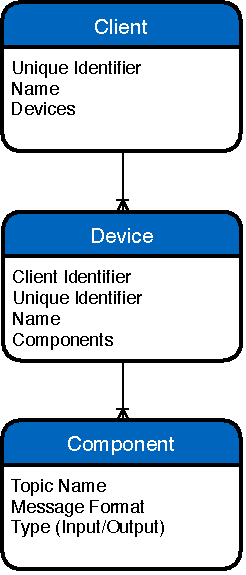
\includegraphics[width=3cm]{figures/ubii_er_client.pdf}
    \caption{The client components.}
    \label{fig:ubii_er_client}
  \end{subfigure}%
  \begin{subfigure}{.5\textwidth}
    \centering
    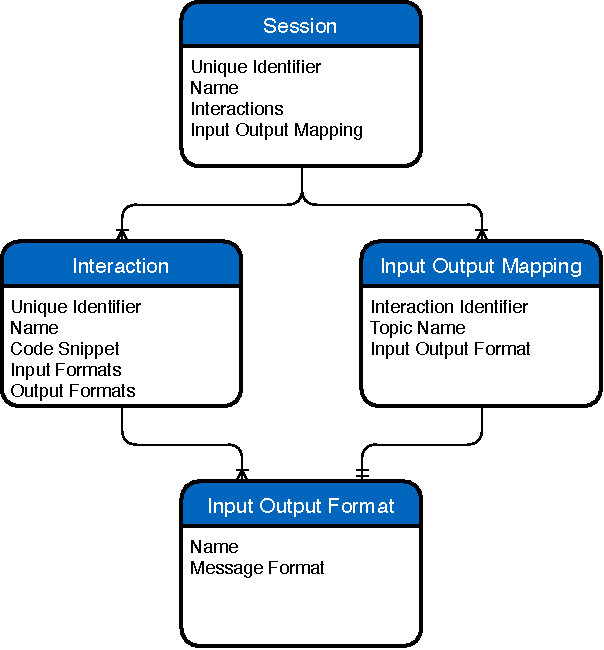
\includegraphics[width=7cm]{figures/ubii_er_server.pdf}
    \caption{The server components.}
    \label{fig:ubii_er_server}
  \end{subfigure}
  \caption{Relationships of the core components in an entity relationship diagram.}
  \label{fig:ubii_er}
\end{figure}



